%% LyX 2.0.3 created this file.  For more info, see http://www.lyx.org/.
%% Do not edit unless you really know what you are doing.
\documentclass[english]{article}
\usepackage{mathptmx}
\usepackage{helvet}
\usepackage{courier}
\usepackage[T1]{fontenc}
\usepackage[latin9]{inputenc}
\usepackage{geometry}
\geometry{verbose,tmargin=2.54cm,bmargin=2.54cm,lmargin=2.54cm,rmargin=2.54cm}
\usepackage{graphicx}

\makeatletter

%%%%%%%%%%%%%%%%%%%%%%%%%%%%%% LyX specific LaTeX commands.
%% Because html converters don't know tabularnewline
\providecommand{\tabularnewline}{\\}

\makeatother

\usepackage{babel}
\begin{document}

\title{Comparison and analysis of transcription factor binding sites}


\author{Colin Diesh}


\date{Senior Thesis Project, Fall 2012\\
$\,$\\
First semester final report - Outline}
\maketitle
\begin{abstract}
Transcription factors are proteins which recognize and bind to short
DNA sequences, and they can play an important role in regulating DNA
transcription. Comparing transcription factor binding sites from different
experiments can show functional differences and similarities, however
binding sites have been shown to vary significantly even from closely
related individuals. Zheng et al. characterized transcription factor
binding variations by using a normalized difference score to find
'variable binding regions' across different experiments. We use the
normalized difference score from multiple experiments and we also
use the DNA alignment from different genomes in order to classify
binding sites. 
\end{abstract}

\section{Background}

Protein-DNA interactions play an important role in gene regulation,
and chromatin immunoprecipitation (ChIP) is a methodology for analyzing
these interactions. Antibodies that bind to transcription factors
or histone modifiers are used to immunoprecipitate the protein-DNA
complexes. Using chromatin immunoprecipitation and high throughput
sequencing (ChIP-seq) or oligonucleotide tiling arrays (ChIP-chip)
we can identify transcription factor binding sites. We search for
peaks in the data which corresponds to an enrichment of ChIP in the
sequences. Comparing ChIP data from multiple experiments is important
to identify functional similarities and differences. Here we will
look at some background papers in the field\\



\subsection{Tissue specific transcriptional regulation has diverged significantly
between human and mouse (Odom, Dowell et al.)}
\begin{enumerate}
\item Odom, Dowell et al. used ChIP-chip tiling arrays to analyze binding
site differences in human and mouse hapetocytes (liver tissue). 
\item They used orthologous genes in human and mouse, and they created tiling
arrays from the gene promoter regions
\item They proposed two approaches for data anlysis

\begin{enumerate}
\item - Gene centric approach for ChIP

\begin{enumerate}
\item Classify binding as true/false for each gene (tiling array as a whole)
\item Similar to Zheng et al. by identifying target genes 
\end{enumerate}
\item - Peak centric approach

\begin{enumerate}
\item Classify peaks within tiling array
\item Find 'peaks' using ChIP-chip and compare aligned sites
\item Peaks as conserved, turnover, gain/loss, or unaligned\\
\includegraphics[scale=0.6]{peak_classification}\\
Figure 1. Transcription factor binding sites are classified in terms
of DNA alignment (Odom, Dowell et al. 2007)\\

\item Odom, Dowell results many shared binding sites are not aligned (60\%+)\\
\\
\begin{tabular}{|c|c|c|c|c|}
\hline 
Shared binding sites & FOXA2  & HNF1A & HNF4A & HNF6\tabularnewline
\hline 
\hline 
Binding sites aligns & 34\% & 41\%  & 23\% & 30\%\tabularnewline
\hline 
Binding sites do not align & 39\% & 31\% & 38\%  & 41\%\tabularnewline
\hline 
No alignment & 28\% & 28\% & 38\%  & 30\%\tabularnewline
\hline 
\end{tabular}\\
\\
Table 1. Percent of binding sites that align from different transcription
factors in human and mouse hepatocytes
\end{enumerate}
\end{enumerate}
\item Questions about Odom, Dowell

\begin{enumerate}
\item How can we use their results to answer questions about more similar
functional comparisons. ChIP-seq where sequence comparison is important
for ChIP-seq sequence similarity?
\end{enumerate}
\end{enumerate}

\subsection{Zheng et al. \textendash{} Genetic analysis of transcription factor
binding variation in yeast}
\begin{enumerate}
\item Zheng et al. analyzed binding sites from many yeast ChIP-experiments
using and found potential sources of binding site differences

\begin{enumerate}
\item They first calculated a normalized difference score for ChIP-seq which
does background subtraction and normalization to get the 'binding
signal'
\item Then they analyzed the variation of normdiff across all experiments
to identify cis- and trans- factors contributing to binding site variations

\begin{enumerate}
\item They found that cis-factors, which are DNA changes that were identified
using genetic markers and alignments, were the main source of binding
variations across genomes\\
\\
\includegraphics[scale=0.6]{consensus3}\\
Figure 2. Modifications to DNA motifs in the yeast population correlated
with variable transcription factor binding (Zheng et al, 2010)

\begin{enumerate}
\item They used a 'single marker regression' to associate variable binding
regions with genetic markers and found that 85\% of variable binding
regions in a genetic marker regression laid cis to a genetic marker,
and the effect size was greater for cis-factors than trans-factors
\item Note: see methods/approach for how the marker regression is important
for our goals
\end{enumerate}
\item Zheng et al. also found trans-factors, defined by genetic markers
far away from the binding sites, that were associated with binding
variations (AMN1, FLO8)
\end{enumerate}
\end{enumerate}
\end{enumerate}

\section{Method and approach}

We use ChIP-seq data gathered from two seperate yeast strains (S288c
and YJM789) and then we used alignment of DNA sequences to try to
find conserved transcription factor binding sites that other algorithms
did not identify. We used a normalized difference score that was defined
by Zheng et al. to identify conserved binding sites, and we proposed
modifications to consider multiple genomes concurrently.


\subsection{Normalized difference scores}

The normalized difference (NormDiff) score is a useful statistic for
comparing ChIP-seq data that uses background subtraction and normalization
to obtain the ChIP-seq binding signal. The NormDiff score from Zheng
et al. uses a simple random model for ChIP-seq ($A$) and control
($B$) defined as

\begin{eqnarray*}
A & \sim & Poisson(f+g)\\
B & \sim & Poisson(cg)
\end{eqnarray*}


Where- 

$f$ represents the binding signal

$g$ represents the background noise

$c$ is a scaling factor between $A$ and $B$\\


Then, the NormDiff $Z$ is defined for each genome position $x_{i}$
as 

\[
Z(x_{i})=\frac{A(x_{i})-B(x_{i})/c}{\sigma}
\]
 

Then the scaling factor $c$ is estimated as the median ratio of $A/B$
and the variance $\sigma$ is estimated from the maximum variance
of $\sqrt{A+B/c^{2}}$ in a local window. Then, the background score
is where $Z~Normal(0,1)$ and deviations from the norm are caused
by the strong ChIP-seq binding signals. 

\includegraphics[scale=0.3]{Rplot08}\includegraphics[scale=0.3]{Rplot05_2}

Figure 3. (left) Kernel density plot of NormDiff for whole genome
shows approx. normal distribution of background reads. (right) Q-Q
Plot shows that NormDiff scores ChIP-seq binding signals are highly
different from the background 


\subsection{Finding conserved binding sites}

We identified a set of high confidence binding sites in ChIP-seq data
using MACS (Zhang et al, 2008). However, we found that there was evidence
for shared binding sites from both parents at this threshold. We compared
the NormDiff scores from binding sites in one experiment with the
syntenic regions of the other experiments, and we found that there
was considerable overlap between the NormDiff scores of the shared
binding sites with the sites that were not called by MACS (Figure
4)

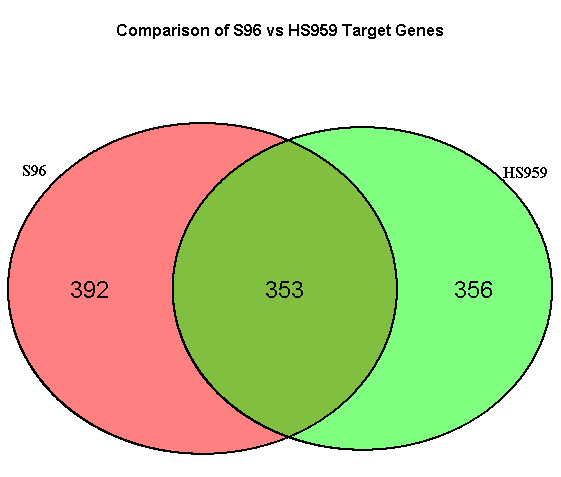
\includegraphics[scale=0.4]{image7}

Figure 4. The NormDiff scores from binding sites found in one ChIP-seq
experiment compared with the NormDiff score of the syntenic region
from a different experiment. Shared binding sites are identified as
orange, and binding sites specific to S96 and HS959 are blue and purple
respectively.


\subsection{Results}
\begin{itemize}
\item We found 42 new binding sites in HS959 with P<0.05 that were conserved
in S96 that were not identified by MACS. Also 4 of these binding sites
were conserved with P<0.01
\item We found 76 binding sites in S96 with P<0.05 that were conserved in
HS959, and 13 of these binding sites were conserved with P<0.01 
\item To evaluate the significance of these findings, we evaluated peaks
in S96 using normalized difference scores and identified 98\% (885/897)
of the binding sites that MACS identifies at P<0.05 confidence level,
and 60\% (563/897) binding sites at a P<0.01. 
\item In HS959 we identified 85\% (729/824) of the same peaks that MACS
identifies at a 0.05 confidence level and 46\% (365/824) peaks at
P<0.01\\
\includegraphics[scale=0.4]{Rplot25}\\
Figure 5. The maximum average NormDiff score is used to identify additional
binding sites that are conserved in each experiment. 
\end{itemize}

\section{Discussion}

We identified some additional evidence for conserved binding sites
by using the normalized difference score that were not identified
by peak finding algorithms. Our work could be extended to use more
sophisticated statistical models. For example, we considered modifying
NormDiff scores to use data from multiple experiments in order to
find conserved binding sites. The additive and subtractive NormDiff
scores find conserved and differential expression. 


\subsection{Modified normdiff score}

We propose using a modified NormDiff score that uses data from multiple
experiments. A NormDiff score that adds data from two experiments,
A1,B1,A2, and B2 can be defined as \\
\[
Z_{add}(x_{i})=\frac{(A_{1}-B_{1}/c_{1})+(A_{2}-B_{2}/c_{2})}{\sigma}
\]


Then the scaling factors $c_{1}$and $c_{2}$ are estimated from data,
and the variance is $\sigma=\sqrt{A_{1}+B_{1}/c_{1}^{2}+A_{2}+B_{2}/c{}_{2}^{2}}$ 

A NormDiff score that subtracts data from two experiments could also
be defined as
\[
Z_{sub}(x_{i})=\frac{(A_{1}-B_{1}/c_{1})-(A_{2}-B_{2}/c_{2})}{\sigma}
\]


The variance for $Z_{sub}$ would be the same as the variance for
$Z_{add}$. It is possible that adding and subtracting NormDiff scores
might be able to help in identifying conserved and differential binding.
For example, if the subtractive score is small but the additive score
is large, then the binding site is likely to be conserved in both
experiments.\\


\includegraphics[scale=0.4]{Rplot28}

Figure 6. $Z_{add}$ vs. $Z_{sub}$ for S96 and HS959. This plot is
similar to a MA plot because log product and log ratio are similar
to adding and subtracting the scores. The unique and shared binding
sites are colored

\includegraphics[scale=0.4]{Rplot05}

Figure 7. MA-plot of shared and unique peaks from S96 and HS959. Unique
peaks to S96 colored green, unique peaks to HS959 colored red, shared
peaks from both colored blue.

.


\subsection{Drawbacks of our approach}

Our approach tries to find evidence for conserved binding sites by
analyzing data using normalized difference scores. Our approach gives
some evidence of peaks with high confidence P-values, such as our
results of finding new peaks with P<0.01. However, these findings
have much less confidence than thresholds set by MACS (P<1e-5). Given
that our technique for calculating P-value is similar to MACS, by
finding large deviations from the background distribution, our results
are not very strong. 

One of the reasons for having less confidence in P-values is because
NormDiff uses control data for background subtraction. MACS on the
other hand uses only ChIP-seq data to calculate P-values, and does
not subtract control data. Instead MACS uses control data for filtering
and empirical FDR. Because of this, finding high confidence peaks
relies on using the FDR in MACS, and it is actually possible to use
FDR to adjust the P-value from MACS to be more leniant. So, because
the weakness of NormDiff to find conserved binding sites in ChIP-seq
data with confidence, it seems unproductive to do this analysis. 


\subsection{Applications of NormDiff}

NormDiff scores have interesting applications for finding conserved
and differential binding sites besides our method. One marked example
was the use of the NormDiff score to find variable binding regions
across many ChIP-seq experiments by Zheng et al. Another example is
what Zheng et al. describe as a ``transgressive score'' which is
used to evaluate whether binding sites from yeast cross strains were
inherited from their parents. The transgressive score analyzes the
variance of normdiff scores across all children versus the difference
of the parents -- it is defined as 
\[
\frac{var(Z)}{Z_{parent1}-Z_{parent2}}
\]


They say that if the transgressive score is low, then the binding
site is inherited from one of the parents, and so in some sense it
was conserved. However, if the transgressive score is high then the
binding site was an extreme phenotype not found in either parent.
Their analysis shows in yeast that some even lowly expressed peaks
might be called transgressive because they are not conserved with
the same strength of the parents' binding sites. 

\includegraphics[scale=0.6]{untitled4}

Figure 8. Comparison of the signal tracks from different ChIP-seq
scores shows that some experiments. ``ChIP-Seq signal tracks showing
Ste12-binding sites that segregate in a Mendelian (left) or transgressive
(middle and right) fashion. The colour indicates genotype background
in the depicted regions: red (S96), green (HS959). Asterisks indicate
peaks of interest''\\



\section{Next steps}


\subsection{Problem statement}
\begin{enumerate}
\item One of the main results tools from Zheng et al. is the use of NormDiff
\item NormDiff is used to find 'variable binding regions', where normdiff
scores have a high degree of variability across experiments
\item Then, variable binding regions are linked with genetic markers using
'single marker regression'

\begin{enumerate}
\item This marker technique is used to analyze quantitative trait loci (QTL)
and to identify cis-factors and trans-factors
\item The genetic markers indicate SNP and indel modifications, but the
marker regression does not explicitely address the alignment of binding
sites
\end{enumerate}
\item We want to classify binding sites as being having conserved, gain/loss,
turnover, and unaligned alignments similar to Odom, Dowell et al.
\item Furthermore, Zheng et al say that 84\% of variable binding regions
overlap the binding sites, so this our classification would also characterize
many of the variable binding regions.
\end{enumerate}
This new problem of classifying binding sites can help quantify binding
site similarity and differences. However, our problem that we addressed
in our previous application was for finding conserved binding sites.
Therefore, we used only aligned ChIP-seq data to look for additional
signal in the noise to find binding sites that weren't called by other
algorithms. My problem statement here is meant to show a broader perspective
however.


\section{Conclusion}

Normalized difference scores have a variety of applications for comparing
ChIP-seq experiments. We used normalized difference scores to find
conserved binding sites in multiple experiments. However, there are
some significant challenges in this analysis. We will extend our methods
to classify binding sites according to their alignment similar to
Odom, Dowell et al and this will improve our ability to characterize
'variable binding regions' also. Overall, these methods will be able
to better identify binding site differences an similarities. 
\end{document}
